% Book 4, Year 2, chapter 12 -- Caches and the memory hierarchy.
% Provenance (never printed): sources/book4/BRIEFS.md, chapter 12.
\chapter{Caches and the Memory Hierarchy}\label{ch:b2:caches}

Here is a program that adds up the $4096 \times 4096$ integers of a matrix twice: once row by row, once column by
column. The two loops perform the same additions on the same numbers and print the same sum.

\omcode{code/bachelor-2/12-caches/listings/rows_cols.c}{23}{35}{The same sum, in two orders}

\omoutput{code/bachelor-2/12-caches/outputs/rows_cols.txt}{One run on the author's laptop, compiled with
\code{-O2}.}\label{out:b2:caches:hook}

The column order is about thirty times slower. Nothing in the instructions explains it: both loops execute one load
and one addition per element. The difference lies in where the loaded integers come from. A load that finds its word
in a small memory next to the processor takes about a nanosecond; a load that must go to the memory modules on the
motherboard takes more than a hundred. This chapter explains what these small memories are, how they decide what to
keep, how to count their misses with a simulator fed by \code{rv}, and how to write code that they serve well.

\begin{recall}
Book 1: the memory (RAM) holds the running programs and their data and is emptied when the power goes off; a disk
keeps files. Book 3: a process's memory is a sequence of bytes with addresses; a two-dimensional C array is stored
row after row, so that \code{a[i][j]} of an $n \times m$ array lies at offset $(i m + j)$ times the size of an
element. \cref{ch:b2:assembly-and-calling-convention}: \code{lw} and \code{sw} compute an address and access one
word. \cref{ch:b2:processor-and-pipelining}: the memory stage of the pipeline was assumed to take one cycle.
\end{recall}

\section{Locality and the memory hierarchy}\label{sec:b2:caches:hierarchy}

The previous chapter assumed that a load takes one cycle. A memory that is both large and that fast cannot be
built: a larger memory has longer wires and more cells to select from, and the memory chips sit centimetres away
from the processor. What can be built is a small fast memory beside a large slow one. It pays because programs do
not use their addresses at random.

\begin{definition}[Temporal locality, spatial locality]\label{def:b2:caches:locality}
A program has \emph{temporal locality}\index{temporal locality} when an address it has just used is likely to be
used again soon, and \emph{spatial locality}\index{spatial locality} when the addresses near an address it has just
used are likely to be used soon.
\end{definition}

A loop has both: its instructions are fetched again at every turn (temporal), and a walk along an array uses
consecutive addresses (spatial). The row-order sum of the hook has \omterm{def:b2:caches:locality}{spatial locality}; the column order jumps
$4096 \times 4 = 16\,384$ bytes at every step and has none, as long as a column does not fit in the fast memory.

\begin{definition}[Memory hierarchy]\label{def:b2:caches:hierarchy}
A \emph{memory hierarchy}\index{memory hierarchy} is a sequence of memories, each larger and slower than the one
before it, where each level keeps copies of the parts of the next level that were used recently. From the processor
outwards: the registers, two or three levels of \omterm{def:b2:caches:cache}{cache}, the main memory, and the disks.
\end{definition}

The levels can be measured from a program. The trick is to make every load depend on the one before, so that the
processor cannot overlap them: a buffer is filled with pointers that form a single random cycle through its 64-byte
blocks, and the program follows the pointers. The time per step is then the time of one load, and it depends on
which level holds the buffer.

\omcode{code/bachelor-2/12-caches/listings/sweep.c}{23}{47}{Following a random cycle of pointers through buffers of
growing size}

\omoutput{code/bachelor-2/12-caches/outputs/sweep.txt}{One run on the author's laptop: the time of a load, by the size
of the buffer it is taken from.}\label{out:b2:caches:sweep}

\begin{omfigure}
\begin{tikzpicture}
\begin{axis}[omrecord, width=0.9\linewidth, height=6cm, xmode=log, log basis x=2, ymode=log,
    xlabel={size of the buffer (KiB)}, ylabel={ns per load},
    xtick={4,32,256,2048,16384,131072}, xticklabels={4,32,256,2\,048,16\,384,131\,072},
    ytick={1,2,5,10,20,50,100,200}, yticklabels={1,2,5,10,20,50,100,200}, ymin=0.7, ymax=300]
  \addplot[omDef, thick, mark=*, mark size=1.3pt] table[x=kib, y=ns]
    {code/bachelor-2/12-caches/figures/sweep.dat};
  \draw[omThm, dashed] (axis cs:48,0.7) -- (axis cs:48,300) node[pos=0.93, left, font=\scriptsize] {L1};
  \draw[omThm, dashed] (axis cs:2048,0.7) -- (axis cs:2048,300) node[pos=0.93, left, font=\scriptsize] {L2};
  \draw[omThm, dashed] (axis cs:24576,0.7) -- (axis cs:24576,300) node[pos=0.93, left, font=\scriptsize] {L3};
\end{axis}
\end{tikzpicture}
\par\smallskip{\small The measurements of \cref{out:b2:caches:sweep}, on logarithmic scales. The dashed lines are the
capacities of the laptop's three \omterm{def:b2:caches:cache}{caches}, as \code{getconf} reports them below. Each time the buffer outgrows a
level, the time of a load rises to that of the next.}
\end{omfigure}

The curve has four plateaus. Up to 32 KiB a load takes about one nanosecond; from 64 KiB to 1 MiB, about four;
around 4 MiB, about twenty; beyond 16 MiB, about 150. A step need not fall exactly at a capacity: a \omterm{def:b2:caches:cache}{cache} is shared
with other programs, and when random addresses cover thousands of memory pages the processor's translation of
addresses, a subject of operating systems, adds misses of its own. Registers do not appear in the sweep: they are
read within the cycle of the instruction that names them. Disks are much slower again, and a program reaches them
only through the operating system, as \cref{ch:b2:files-pipes-signals} shows.

\begin{omfigure}
\begin{tikzpicture}[font=\small, lev/.style={draw, fill=omDef!#1, minimum height=8mm, align=center}]
\node[lev=40, minimum width=2.6cm] (r) at (0,4.0) {registers};
\node[lev=30, minimum width=4.0cm] (l1) at (0,3.2) {L1 cache, 48 KiB};
\node[lev=22, minimum width=5.4cm] (l2) at (0,2.4) {L2 cache, 2 MiB};
\node[lev=15, minimum width=6.8cm] (l3) at (0,1.6) {L3 cache, 24 MiB};
\node[lev=8, minimum width=8.2cm] (m) at (0,0.8) {main memory, gigabytes};
\node[lev=3, minimum width=9.6cm] (d) at (0,0) {solid-state or hard disk};
\node[anchor=west, font=\scriptsize] at (5.2,4.0) {within the cycle};
\node[anchor=west, font=\scriptsize] at (5.2,3.2) {about 1 ns};
\node[anchor=west, font=\scriptsize] at (5.2,2.4) {about 4 ns};
\node[anchor=west, font=\scriptsize] at (5.2,1.6) {about 20 ns};
\node[anchor=west, font=\scriptsize] at (5.2,0.8) {about 150 ns};
\node[anchor=west, font=\scriptsize] at (5.2,0) {through the system};
\draw[-{Stealth}] (-5.4,4.2) -- node[left, align=right, font=\scriptsize] {smaller,\\ faster} (-5.4,2.6);
\draw[-{Stealth}] (-5.4,1.8) -- node[left, align=right, font=\scriptsize] {larger,\\ slower} (-5.4,0.0);
\end{tikzpicture}
\par\smallskip{\small The \omterm{def:b2:caches:hierarchy}{memory hierarchy} of the author's laptop. The capacities are those of \code{getconf}; the
times are the plateaus of \cref{out:b2:caches:sweep}, the time of one load served by that level.}
\end{omfigure}

\omimg{book4/memory-modules-rear.jpg}{0.5\linewidth}{The back of two laptop memory modules of 8\,GB each. The gold
contacts along the lower edge plug into the motherboard; an access that misses in every \omterm{def:b2:caches:cache}{cache} is served by modules
like these. Photograph: ITEagle Europe -- Sebastiaan Broekhoven, CC BY-SA 4.0.}

% ledger: b2:cache-wilkes, b2:cache-360-85
\begin{history}[A slave memory]
In April 1965 M.~V.~Wilkes published a two-page paper proposing a small fast ``slave memory'' that would hold copies
of the words of a large slow main memory most recently used, so that most accesses would be as fast as the small
memory. In 1968 a description of a large commercial computer, the IBM System/360 Model 85, called such a buffer a
\emph{\omterm{def:b2:caches:cache}{cache}}, and the word stayed.
\end{history}

\section{Direct-mapped caches}\label{sec:b2:caches:direct}

\begin{definition}[Cache, line, hit, miss]\label{def:b2:caches:cache}
A \emph{cache}\index{cache} is a small fast memory that holds copies of blocks of a larger memory. The block it
moves at once, $B$ bytes with $B$ a power of two at an address multiple of $B$, is a \emph{cache line}\index{cache
line}. An access whose line is in the cache is a \emph{hit}\index{hit}; otherwise it is a \emph{miss}\index{miss},
and the line is fetched from the next level. The \emph{hit rate}\index{hit rate} of a run is its number of hits
divided by its number of accesses, and the \emph{miss ratio} is one minus the hit rate.
\end{definition}

The hook's laptop has 64-byte lines: the first load of a row brings 16 integers, and the next 15 loads \omterm{def:b2:caches:cache}{hit}. That is
why the row-order sum is fast: it misses once every 16 integers. A \omterm{def:b2:caches:cache}{cache} must decide, for each line, where it may be
stored and how to find it again. The simplest rule gives every line exactly one place.

\begin{definition}[Tag, index and offset fields]\label{def:b2:caches:fields}
In a \omterm{def:b2:caches:cache}{cache} of $S$ sets of lines of $B$ bytes, with $S$ and $B$ powers of two, an address is cut into three fields:
the \emph{offset field}\index{offset field}, its low $\log_2 B$ bits, which select a byte in the line; the
\emph{index field}\index{index field}, the next $\log_2 S$ bits, which select the set; and the \emph{tag
field}\index{tag field}, the remaining high bits, stored beside the line to tell which of the many lines that share
the set is there.
\end{definition}

\begin{definition}[Direct-mapped, set-associative, fully associative]\label{def:b2:caches:mapping}
A \omterm{def:b2:caches:cache}{cache} is \emph{direct-mapped}\index{direct-mapped cache} when each set holds one line, so that a line can be in
one place only; \emph{$A$-way set-associative}\index{set-associative cache} when each set holds $A$ lines, any of
which may receive a line of that set; and \emph{fully associative}\index{fully associative cache} when there is one
set, so that any line can go anywhere.
\end{definition}

\begin{proposition}[Field widths]\label{prop:b2:caches:fields}
A \omterm{def:b2:caches:cache}{cache} of $C$ bytes, $A$-way set-associative with lines of $B$ bytes, all powers of two, has $S = C / (A B)$ sets.
With $w$-bit addresses, its \omterm{def:b2:caches:fields}{offset field} has $\log_2 B$ bits, its \omterm{def:b2:caches:fields}{index field} $\log_2 S$ bits, and its \omterm{def:b2:caches:fields}{tag field}
$w - \log_2 S - \log_2 B$ bits.
\end{proposition}

\begin{proof}
The \omterm{def:b2:caches:cache}{cache} holds $C / B$ lines, grouped $A$ per set, hence $S = C/(AB)$ sets. A byte in a line of $B = 2^b$ bytes is
named by $b$ bits, a set among $S = 2^s$ by $s$ bits, and the tag keeps all the other bits, because two lines that
share an index differ only there: knowing the set and the tag, the line's address is the tag, then the index, then
$b$ zero bits.
\end{proof}

\begin{omfigure}
\begin{bytefield}[bitwidth=0.95em, bitheight=6mm]{32}
\bitheader[endianness=big]{0,4,5,8,9,31} \\
\bitbox{23}{tag: the remaining 23 bits} & \bitbox{4}{index} & \bitbox{5}{offset}
\end{bytefield}
\par\smallskip{\small The fields of a 32-bit address for a \omterm{def:b2:caches:mapping}{direct-mapped cache} of 512 bytes with 32-byte lines:
16 sets, so 4 index bits and 5 offset bits. The same address cut for another \omterm{def:b2:caches:cache}{cache} gives other fields.}
\end{omfigure}

The simulator \code{cache.py} implements the three kinds at once: \code{ways = 1} gives a \omterm{def:b2:caches:mapping}{direct-mapped cache},
\code{ways} equal to the number of lines a \omterm{def:b2:caches:mapping}{fully associative} one. Each set is an ordered dictionary from tags to a
``dirty'' flag, kept in the order of last use; the flag and the order serve in the next section.

\omcode{code/bachelor-2/12-caches/listings/cache.py}{5}{17}{The \omterm{def:b2:caches:cache}{cache}'s shape}\label{lst:b2:caches:shape}

\omcode{code/bachelor-2/12-caches/listings/cache.py}{19}{46}{Splitting an address, and one
access}\label{lst:b2:caches:access}

\begin{method}[Tracing a direct-mapped cache by hand]\label{met:b2:caches:trace}
Start from an empty \omterm{def:b2:caches:cache}{cache}. For each address: write it in binary and cut it into tag, index and offset; look at the
set given by the index; if it holds the same tag, it is a \omterm{def:b2:caches:cache}{hit}; otherwise it is a \omterm{def:b2:caches:cache}{miss}, and the set now holds the new
tag, whatever it held before. Keep a table with one row per set and update it at each \omterm{def:b2:caches:cache}{miss}.
\end{method}

A \omterm{def:b2:caches:cache}{cache} of 256 bytes with 16-byte lines has 16 sets: 4 offset bits, 4 index bits. Here is a trace of eight
accesses:

\omoutput{code/bachelor-2/12-caches/outputs/run_hand_trace.txt}{A \omterm{def:b2:caches:mapping}{direct-mapped cache}, access by access; the
last line gives the tag held by each valid set.}\label{out:b2:caches:hand}

\code{0x004} \omterm{def:b2:caches:cache}{hits} because \code{0x000} brought the whole line \code{0x000} to \code{0x00f}. \code{0x100} has the
same index as \code{0x000} and another tag: it evicts it, and the following \code{0x000} misses again, although the
\omterm{def:b2:caches:cache}{cache} has fourteen empty sets. Two lines that keep evicting each other while space is free elsewhere are the
weakness of the direct mapping.

\begin{omfigure}
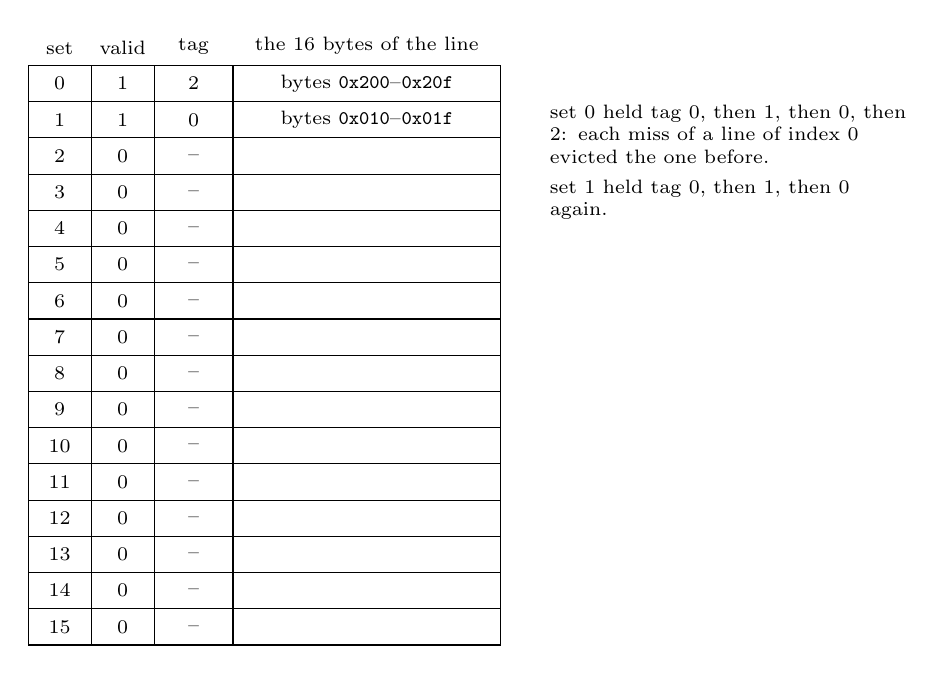
\begin{tikzpicture}[font=\scriptsize, cell/.style={draw, minimum height=4.6mm, inner sep=1pt}]
\foreach \i in {0,...,15} {
  \node[cell, minimum width=8mm] at (0,-0.46*\i) {\i};
  \node[cell, minimum width=8mm] at (0.8,-0.46*\i) {\ifnum\i<2 1\else 0\fi};
  \node[cell, minimum width=10mm] at (1.7,-0.46*\i) {\ifnum\i=0 2\else\ifnum\i=1 0\else --\fi\fi};
  \node[cell, minimum width=34mm] at (3.9,-0.46*\i)
    {\ifnum\i=0 bytes \texttt{0x200}--\texttt{0x20f}\else\ifnum\i=1 bytes \texttt{0x010}--\texttt{0x01f}\else\fi\fi};
}
\node[above] at (0,0.25) {set}; \node[above] at (0.8,0.25) {valid}; \node[above] at (1.7,0.25) {tag};
\node[above] at (3.9,0.25) {the 16 bytes of the line};
\node[anchor=west, align=left, text width=4.6cm] at (6.1,-1.0) {set 0 held tag 0, then 1, then 0, then 2: each
miss of a line of index 0 evicted the one before.\\[3pt] set 1 held tag 0, then 1, then 0 again.};
\end{tikzpicture}
\par\smallskip{\small The \omterm{def:b2:caches:cache}{cache} after the trace of \cref{out:b2:caches:hand}. Only two of its sixteen sets were
ever used; the valid bit tells an empty set from a set holding tag 0.}
\end{omfigure}

The same simulator can be fed with real programs. \code{matrix_sum.S} fills a $32 \times 32$ matrix of words and
sums it in the order its input chooses; \code{trace_demo.py} runs it on \code{rv} and keeps the address of every
load, through the \code{trace} callback met in \cref{ch:b2:processor-and-pipelining}. Like the short programs of
\cref{ch:b2:assembly-and-calling-convention}, its \code{main} uses \code{s} registers without saving them, which only
\code{rv}, where nothing runs after \code{main}, tolerates.

\omcode{code/bachelor-2/12-caches/listings/matrix_sum.S}{25}{40}{The sum: \code{s2} chooses which counter is the
row}

\omcode{code/bachelor-2/12-caches/listings/trace_demo.py}{6}{21}{The loads of a run, through a 1 KiB \omterm{def:b2:caches:mapping}{direct-mapped
cache} with 32-byte lines}

\omoutput{code/bachelor-2/12-caches/outputs/run_trace.txt}{Row order and column order on the
simulator.}\label{out:b2:caches:trace}

In row order the addresses step by 4 and each 32-byte line serves 8 loads: 128 misses for 1024 loads, a \omterm{def:b2:caches:cache}{miss} ratio
of $1/8$. In column order they step by 128 bytes, a whole row; every load misses. Yet the matrix's 32 rows need only
32 lines in a column, and the \omterm{def:b2:caches:cache}{cache} has 32 lines. \cref{sec:b2:caches:three-c} finds out why they do not stay.

\section{Associative caches and write policies}\label{sec:b2:caches:associative}

An $A$-way \omterm{def:b2:caches:cache}{cache} lets $A$ lines of the same index live together. On a \omterm{def:b2:caches:cache}{miss} in a full set, one of them must go.

\begin{definition}[Replacement policy, LRU]\label{def:b2:caches:lru}
The \emph{replacement policy}\index{replacement policy} of a \omterm{def:b2:caches:mapping}{set-associative cache} chooses which line of a full set
a \omterm{def:b2:caches:cache}{miss} evicts. The \emph{least recently used}\index{least recently used} (LRU) policy evicts the line whose last
access is the oldest.
\end{definition}

In hardware, a 2-way set needs one bit to remember which of its two lines is older; the simulator keeps each set's
tags in order of use and moves a tag to the end on every \omterm{def:b2:caches:cache}{hit} (\code{move_to_end}), so that the first tag is always
the one to evict (\code{popitem(last=False)}).

\begin{omfigure}
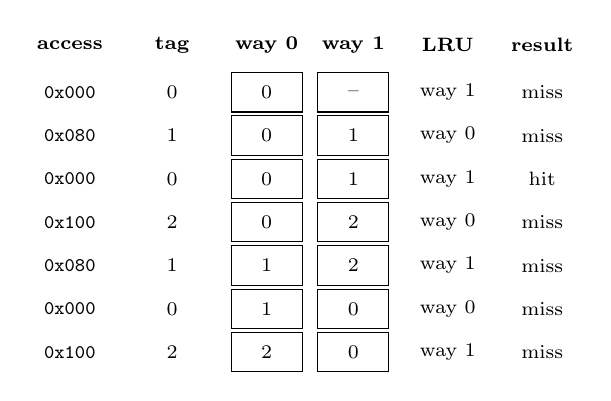
\begin{tikzpicture}[font=\scriptsize, c/.style={draw, minimum width=9mm, minimum height=5mm, inner sep=1pt},
  hd/.style={font=\scriptsize\bfseries}]
\node[hd] at (0,0.6) {access}; \node[hd] at (1.3,0.6) {tag}; \node[hd] at (2.5,0.6) {way 0};
\node[hd] at (3.6,0.6) {way 1}; \node[hd] at (4.8,0.6) {LRU}; \node[hd] at (6.0,0.6) {result};
\foreach [count=\r] \a/\t/\wa/\wb/\l/\res in {
    0x000/0/0/--/1/miss, 0x080/1/0/1/0/miss, 0x000/0/0/1/1/hit, 0x100/2/0/2/0/miss,
    0x080/1/1/2/1/miss, 0x000/0/1/0/0/miss, 0x100/2/2/0/1/miss} {
  \node at (0,-0.55*\r+0.55) {\texttt{\a}}; \node at (1.3,-0.55*\r+0.55) {\t};
  \node[c] at (2.5,-0.55*\r+0.55) {\wa}; \node[c] at (3.6,-0.55*\r+0.55) {\wb};
  \node at (4.8,-0.55*\r+0.55) {way \l}; \node at (6.0,-0.55*\r+0.55) {\res};
}
\end{tikzpicture}
\par\smallskip{\small Set 0 of a 256-byte 2-way \omterm{def:b2:caches:cache}{cache} with 16-byte lines (8 sets, so the tag is the address shifted
right by 7), after each access of a trace. The LRU bit names the way to evict at the next \omterm{def:b2:caches:cache}{miss}. The third access
\omterm{def:b2:caches:cache}{hits}; from then on each line is evicted just before it is needed again.}
\end{omfigure}

Stores raise a second question: when the \omterm{def:b2:caches:cache}{cache} holds a copy of a line, a store changes the copy, and the memory below
must eventually see the change.

\begin{definition}[Write-through, write-back, write-allocate]\label{def:b2:caches:write}
A \emph{write-through}\index{write-through} \omterm{def:b2:caches:cache}{cache} sends every store to the next level as well. A
\emph{write-back}\index{write-back} \omterm{def:b2:caches:cache}{cache} only changes its copy and marks the line \emph{dirty}; a dirty line is
written to the next level when it is evicted. A \omterm{def:b2:caches:cache}{cache} is \emph{write-allocate}\index{write-allocate} when a store
that misses first brings the line into the \omterm{def:b2:caches:cache}{cache}; otherwise the store goes to the next level and the \omterm{def:b2:caches:cache}{cache} is
unchanged.
\end{definition}

\omterm{def:b2:caches:write}{Write-back} saves traffic when a line is written many times before it leaves: a loop that adds into the same counter a
million times writes memory once. \omterm{def:b2:caches:write}{Write-through} keeps the next level always up to date, at the cost of one memory
write per store. In \code{cache.py}, the value stored in a set's dictionary is the dirty flag: an eviction adds it to
\code{memory_writes}, and a \omterm{def:b2:caches:write}{write-through} \omterm{def:b2:caches:cache}{cache} adds one at every store.

\section{Three kinds of misses}\label{sec:b2:caches:three-c}

\begin{definition}[Compulsory, capacity and conflict misses]\label{def:b2:caches:three-c}
A \omterm{def:b2:caches:cache}{miss} is \emph{compulsory}\index{compulsory miss} when its line was never accessed before: every \omterm{def:b2:caches:cache}{cache} misses it.
It is a \emph{capacity miss}\index{capacity miss} when a \omterm{def:b2:caches:mapping}{fully associative} LRU \omterm{def:b2:caches:cache}{cache} of the same size would also
\omterm{def:b2:caches:cache}{miss} it: the program used more distinct lines since the last use of this one than the \omterm{def:b2:caches:cache}{cache} can hold. Otherwise it
is a \emph{conflict miss}\index{conflict miss}: only the mapping of lines to sets caused it.
\end{definition}

The definition is a recipe: run the trace on the \omterm{def:b2:caches:cache}{cache} and, beside it, on a \omterm{def:b2:caches:mapping}{fully associative} ``shadow'' \omterm{def:b2:caches:cache}{cache} of the
same size, and classify each \omterm{def:b2:caches:cache}{miss} by what the shadow did. \cref{exo:b2:caches:7} writes the classifier; here is its
verdict on the column-order sum, and on a loop that sweeps 33 lines over and over through a \omterm{def:b2:caches:cache}{cache} of 32.

\omoutput{code/bachelor-2/12-caches/outputs/run_three_c.txt}{Misses classified, for three \omterm{def:b2:caches:cache}{caches} of 1 KiB with
32-byte lines.}\label{out:b2:caches:three-c}

In column order, 896 of the 1024 misses are conflicts. A column visits addresses 128 bytes apart; with 32-byte lines
and 32 sets, the index is bits 5 to 9 of the address, and adding 128 adds 4 to it: the 32 lines of a column fall into
the 8 sets whose index is a multiple of 4 (the column's first line decides which multiple), and the other 24 sets
stay empty. Two ways do not help: with 16 sets of two ways, the 32 lines then fall in 4 sets, 8 places for 32 lines. A \omterm{def:b2:caches:mapping}{fully associative cache} of the same
size keeps the 32 lines and misses only on first use. The cyclic sweep shows the opposite case.

\begin{proposition}[A cyclic sweep defeats LRU]\label{prop:b2:caches:cyclic}
A \omterm{def:b2:caches:mapping}{fully associative} LRU \omterm{def:b2:caches:cache}{cache} of $C$ lines, accessed cyclically over $C + 1$ distinct lines $\ell_0, \ell_1,
\dots, \ell_C, \ell_0, \ell_1, \dots$, misses on every access.
\end{proposition}

The proof is \cref{exo:b2:caches:8}; the simulator checks it for several $C$ in the chapter's tests, and the output
above shows it for $C = 32$: 330 accesses, 330 misses. The \omterm{def:b2:caches:mapping}{direct-mapped cache} does better on this sweep, 51 misses,
because it evicts only the line that shares a set with the newcomer: lines $\ell_0$ and $\ell_{32}$ fight over set 0,
and the 31 others stay. LRU, a good policy for most programs, is the worst possible one for a loop just too large for the
\omterm{def:b2:caches:cache}{cache}. The cure is to make the loop's data fit: the 18 misses left even in the \omterm{def:b2:caches:mapping}{direct-mapped cache} are still
capacity misses.

\begin{proposition}[Row and column order]\label{prop:b2:caches:traversal}
Let an $N \times N$ matrix of $w$-byte elements be stored row after row, with each row a whole number of lines of
$B$ bytes, and read once, from a cold \omterm{def:b2:caches:mapping}{fully associative} LRU \omterm{def:b2:caches:cache}{cache} of $C$ lines. In row order the reads \omterm{def:b2:caches:cache}{miss}
$N^2 w / B$ times. In column order they \omterm{def:b2:caches:cache}{miss} $N^2 w / B$ times if $C \ge N$, and $N^2$ times, on every read, if
$C < N$.
\end{proposition}

\begin{proof}
A line holds $B/w$ consecutive elements of one row. In row order each line is read in $B/w$ consecutive accesses: the
first misses (\omterm{def:b2:caches:three-c}{compulsory}) and the others \omterm{def:b2:caches:cache}{hit}, since nothing comes between them. That gives one \omterm{def:b2:caches:cache}{miss} per line, and
the matrix has $N^2 w / B$ lines.
In column order, the element $(i, j)$ and the next element of its line, $(i, j + 1)$, are read $N$ accesses apart.
Between them come the elements $(i + 1, j), \dots, (N - 1, j)$ and $(0, j + 1), \dots, (i - 1, j + 1)$: $N - 1$
elements of $N - 1$ other rows, hence of $N - 1$ distinct lines, each read once. Under LRU the line of $(i, j)$ is
still present after them if and only if the \omterm{def:b2:caches:cache}{cache} holds at least $N$ lines. If $C \ge N$, every line misses only on
its first access; if $C < N$, every access finds its line evicted.
\end{proof}

The hook's matrix has $N = 4096$ rows; a column needs 4096 lines of 64 bytes, 256 KiB, more than the 48 KiB L1. By
the proposition every load of the column order misses in L1, against one in 16 for the row order. In the simulator's
\omterm{def:b2:caches:mapping}{direct-mapped cache} of \cref{out:b2:caches:trace}, $C = N = 32$, but conflicts gave the column order the worst case
anyway.

\section{Code that respects the cache}\label{sec:b2:caches:code}

\begin{definition}[Loop interchange, blocking]\label{def:b2:caches:blocking}
\emph{Loop interchange}\index{loop interchange} swaps two nested loops so that the inner loop walks consecutive
addresses. \emph{Blocking}\index{blocking}, or \emph{tiling}\index{tiling}, cuts an array into tiles small enough to
stay in the \omterm{def:b2:caches:cache}{cache} together, and does all the work on a tile, or on a few tiles, before moving on.
\end{definition}

The product of two $n \times n$ matrices, $C_{ij} = \sum_k A_{ik} B_{kj}$, is the classic case. Written as in the
formula, its inner loop walks $B$ down a column: $n$ doubles, $8n$ bytes apart. Interchanging the two inner loops
makes every inner walk a row walk, for the same additions in another order.

\omcode{code/bachelor-2/12-caches/listings/matmul.c}{17}{36}{The product as written, and with its loops
interchanged}

\omcode{code/bachelor-2/12-caches/listings/matmul.c}{38}{49}{The interchanged product on $64 \times 64$
tiles}\label{lst:b2:caches:blocked}

\omoutput{code/bachelor-2/12-caches/outputs/matmul.txt}{One run on the author's laptop: three loop orders, two
sizes. The check is a sum of entries of $C$, the same for every order.}\label{out:b2:caches:matmul}

The interchange alone makes the $1024 \times 1024$ product about ten times faster. \omterm{def:b2:caches:blocking}{Blocking} is slower than the plain
interchanged loop at this size: the three matrices take 8 MiB each, $B$ fits in the 24 MiB L3, and the processor
fetches the next lines of a row walk ahead of the loads that need them (\emph{prefetching}), so that the row walks
of \code{ikj} rarely wait. At $n = 2048$ each matrix takes 32 MiB, more than the L3. Then \code{ikj} reads the whole
of $B$ from memory for every row of $A$: its time grows about nineteen-fold for eight times the arithmetic. The tiled
version reuses each tile of $B$ for 64 rows of $A$ while it is in \omterm{def:b2:caches:cache}{cache}, and its time grows about eightfold, like the
arithmetic. \omterm{def:b2:caches:blocking}{Blocking} pays when the data no longer fits.

\begin{omfigure}
\begin{tikzpicture}[scale=0.42, font=\scriptsize]
\foreach \ox/\name in {0/C, 9/A, 18/B} {
  \draw[step=2, black!25] (\ox,0) grid (\ox+8,8); \draw (\ox,0) rectangle (\ox+8,8);
  \node at (\ox+4,8.7) {$\name$};
}
\fill[omThm!45] (2,4) rectangle (4,6); \draw[thick] (2,4) rectangle (4,6);
\fill[omDef!35] (9,4) rectangle (17,6); \fill[omDef!70] (13,4) rectangle (15,6); \draw[thick] (9,4) rectangle (17,6);
\fill[omProp!30] (20,0) rectangle (22,8); \fill[omProp!70] (20,2) rectangle (22,4); \draw[thick] (20,0) rectangle (22,8);
\node at (8.5,4) {$=$}; \node at (17.5,4) {$\times$};
\node[align=center, anchor=north] at (3,-0.3) {tile $(ii, jj)$};
\node[align=center, anchor=north] at (13,-0.3) {row of tiles $ii$,\\ tile $kk$ dark};
\node[align=center, anchor=north] at (21,-0.3) {column of tiles $jj$,\\ tile $kk$ dark};
\end{tikzpicture}
\par\smallskip{\small \omterm{def:b2:caches:blocking}{Blocking} the product. The tile of $C$ at $(ii, jj)$ accumulates the products of the tiles of
$A$'s row $ii$ by the tiles of $B$'s column $jj$; at each step $kk$ only three tiles are in use, $3 \times 64 \times
64$ doubles, 96 KiB, which stay in the L2 while they are reused 64 times.}
\end{omfigure}

Records raise the same question at another scale. A catalogue of books stored as an array of structures puts each
book's fields together; a structure of arrays stores each field in its own array. A loop that reads one field of
every record uses all of each line in the second layout and an eighth of it in the first.

\omcode{code/bachelor-2/12-caches/listings/aos_soa.c}{9}{11}{The same records, two layouts}

\omcode{code/bachelor-2/12-caches/listings/aos_soa.c}{32}{40}{The mean price, read from each layout}

\omoutput{code/bachelor-2/12-caches/outputs/aos_soa.txt}{One run on the author's laptop, for $2^{22}$ books.}

Each structure takes 64 bytes, a line's worth, of which the loop reads 8: it moves eight times as many bytes from
memory as the arrays layout, and the measured ratio is about four. The arrays loop is held back by its own chain of
additions, each waiting for the one before (the compiler may not reorder a floating-point sum), rather than by
memory: 2.85\,ms for $2^{22}$ additions is about 0.7\,ns each, while the structures loop moves 256\,MiB in
12.39\,ms, about 22\,GB/s, a bandwidth figure. The array of structures is the right layout when every use of a record reads most of its fields,
as when a book is displayed; the structure of arrays when loops read one field of many records.

A program that tunes itself to the \omterm{def:b2:caches:cache}{cache} needs its parameters, and on Linux the C library reports them.

\begin{dated}{2026}
The \omterm{def:b2:caches:cache}{caches} of the author's laptop, as the C library reports them (sizes in bytes):
\omoutput{code/bachelor-2/12-caches/outputs/cache_params.txt}{The \omterm{def:b2:caches:cache}{cache} parameters, by
\code{getconf}.}\label{out:b2:caches:getconf}
By \cref{prop:b2:caches:fields}, its L1 data \omterm{def:b2:caches:cache}{cache} has $49\,152 / (12 \times 64) = 64$ sets, so 6 offset bits and
6 index bits; the L2 has 2048 sets and the L3 32\,768. Another processor has other numbers; the command shows them.
\end{dated}

\begin{inpractice}[Measuring before tuning]
A loop that is slow because of the \omterm{def:b2:caches:cache}{caches} looks, in the source, exactly like a loop that is not. Measure first, with
the real data size: the matrix product above needed \omterm{def:b2:caches:blocking}{blocking} at one size and not at the other. Then try the cheap
changes in order: walk arrays in the order they are stored, keep the data a loop reads small and together, and only
then cut the work into tiles, whose best size depends on the machine.
\end{inpractice}

\section{Average memory access time}\label{sec:b2:caches:amat}

\begin{definition}[Miss penalty, average memory access time]\label{def:b2:caches:amat}
The \emph{hit time}\index{hit time} of a level is the time of an access it serves; its \emph{miss
penalty}\index{miss penalty} is the extra time of an access it misses, the time to get the line from the levels
below. The \emph{average memory access time}\index{average memory access time} (AMAT) of a run is its total time
spent on memory accesses divided by their number.
\end{definition}

\begin{proposition}[AMAT over several levels]\label{prop:b2:caches:amat}
Let a hierarchy have \omterm{def:b2:caches:cache}{cache} levels $1, \dots, k$ above the main memory. Let $h_i$ be the extra time to reach level
$i$ when level $i - 1$ missed ($h_1$ is the \omterm{def:b2:caches:amat}{hit time} of L1), $m_i$ the \emph{local} \omterm{def:b2:caches:cache}{miss} ratio of level $i$, the
fraction of the accesses reaching level $i$ that \omterm{def:b2:caches:cache}{miss} there, and $T$ the extra time of the main memory. Then
\[
\mathrm{AMAT} = h_1 + m_1\bigl(h_2 + m_2\bigl(h_3 + \cdots + m_{k-1}(h_k + m_k T)\cdots\bigr)\bigr).
\]
\end{proposition}

\begin{proof}
By induction on $k$. Let $P_i$ be the average extra time of an access that reaches level $i$, counted from that
level, with $P_{k+1} = T$. Every access that reaches level $i$ pays $h_i$, and the fraction $m_i$ of them that \omterm{def:b2:caches:cache}{miss}
pays $P_{i+1}$ on top; averaging, $P_i = h_i + m_i P_{i+1}$. Every access reaches level 1, so $\mathrm{AMAT} = P_1$,
and unfolding the recurrence from $P_1$ to $P_{k+1} = T$ gives the formula.
\end{proof}

With the plateaus of \cref{out:b2:caches:sweep} rounded to 1, 4, 20 and 150\,ns, the extra times are $h_1 = 1$,
$h_2 = 3$, $h_3 = 16$ and $T = 130$\,ns. For local \omterm{def:b2:caches:cache}{miss} ratios of 5\,\%, 20\,\% and 30\,\%:
\[
\mathrm{AMAT} = 1 + 0.05\,\bigl(3 + 0.2\,(16 + 0.3 \times 130)\bigr) = 1 + 0.05\,(3 + 0.2 \times 55) = 1.7\ \text{ns}.
\]
Without any \omterm{def:b2:caches:cache}{cache} every access would take 150\,ns, about ninety times longer. The formula also tells where to work:
halving $m_1$ saves $0.35$\,ns here, about as much as removing the trip to main memory altogether ($T = 0$ saves
$0.39$\,ns), and more than twice what removing the L3's own extra time $h_3$ would ($0.16$\,ns).

\section{Exercises}\label{sec:b2:caches:exercises}

\begin{exercise}[$\star$]\label{exo:b2:caches:1}
A \omterm{def:b2:caches:mapping}{direct-mapped cache} of 128 bytes has 16-byte lines. Give its number of sets and the fields of an address, then
trace the accesses \code{0x00}, \code{0x04}, \code{0x08}, \code{0x10}, \code{0x80}, \code{0x00}, \code{0x14},
\code{0x90}, \code{0x1C}, \code{0x84} by \cref{met:b2:caches:trace}. Which misses are \omterm{def:b2:caches:three-c}{compulsory}?
\end{exercise}

\begin{exercise}[$\star$]\label{exo:b2:caches:2}
This simulator takes the index from the top bits of the address instead of the bits just above the offset. Explain
its output on an array of 512 bytes read twice through a 1 KiB \omterm{def:b2:caches:cache}{cache} with 32-byte lines.
\omcode{code/bachelor-2/12-caches/listings/exo_wrong_bits.py}{5}{19}{The index from the wrong bits}
\omoutput{code/bachelor-2/12-caches/outputs/run_wrong_bits.txt}{Correct and wrong mapping.}
\end{exercise}

\begin{exercise}[$\star$]\label{exo:b2:caches:3}
Write \code{dirty_lines(cache)}, the number of lines a \omterm{def:b2:caches:write}{write-back} \code{Cache} would still have to write to memory if
it were emptied now, and \code{total_writes(cache)}. How many memory writes do ten stores to the same word cause in a
\omterm{def:b2:caches:write}{write-back} \omterm{def:b2:caches:cache}{cache}, and in a \omterm{def:b2:caches:write}{write-through} \omterm{def:b2:caches:cache}{cache}?
\end{exercise}

\begin{exercise}[$\star$]\label{exo:b2:caches:4}
Give the fields of a 32-bit address for a 32 KiB 8-way \omterm{def:b2:caches:cache}{cache} with 64-byte lines, and for the laptop's L2 of
\cref{out:b2:caches:getconf}. How many bits of tag does each line of that L2 store?
\end{exercise}

\begin{exercise}[$\star\star$]\label{exo:b2:caches:5}
A 256-byte 2-way LRU \omterm{def:b2:caches:cache}{cache} has 16-byte lines. Trace \code{0x000}, \code{0x100}, \code{0x000}, \code{0x200},
\code{0x100}, \code{0x084}, \code{0x000}, \code{0x300}, \code{0x004}, giving the contents of set 0 after each
access. Then trace the same addresses through a \omterm{def:b2:caches:mapping}{direct-mapped cache} of 256 bytes. Which does better, and why?
\end{exercise}

\begin{exercise}[$\star\star$]\label{exo:b2:caches:6}
This function sums each column of a grid of loan counts, one row per day and one column per book. Interchange its
loops and measure.
\omcode{code/bachelor-2/12-caches/listings/exo_colsums.c}{17}{24}{Column sums, column by column}
\end{exercise}

\begin{exercise}[$\star\star$]\label{exo:b2:caches:7}
Write \code{classify(addresses, size, line, ways)}, which returns the number of misses of a trace and their split into
\omterm{def:b2:caches:three-c}{compulsory}, capacity and conflict misses, by running a \omterm{def:b2:caches:mapping}{fully associative} shadow \omterm{def:b2:caches:cache}{cache} beside the \omterm{def:b2:caches:cache}{cache}. Check that
the three counts add up to the misses.
\end{exercise}

\begin{exercise}[$\star\star$]\label{exo:b2:caches:8}
Prove \cref{prop:b2:caches:cyclic}. Does it still hold for a sweep over $C + 2$ lines? Over $C$ lines?
\end{exercise}

\begin{exercise}[$\star\star$]\label{exo:b2:caches:9}
A transpose writes $b_{ji} = a_{ij}$. Explain why its plain version is slow whichever loop is inside, write a tiled
version and measure it for several tile sizes.
\omcode{code/bachelor-2/12-caches/listings/transpose.c}{16}{21}{The plain transpose of an $8192 \times 8192$ matrix
of \code{int}}
\end{exercise}

\begin{exercise}[$\star\star\star$]\label{exo:b2:caches:10}
In the \omterm{def:b2:caches:mapping}{direct-mapped cache} of \cref{out:b2:caches:trace}, $C = N = 32$, yet the column order misses every time.
Generalise: for an $N \times N$ matrix of 4-byte words, $N$ a power of two at least 8, read in column order through a
\omterm{def:b2:caches:mapping}{direct-mapped cache} of $C$ lines of $B$ bytes, with $C$ and $B$ powers of two, $B \le 4N$, how many sets does a column
use, and when does the column order \omterm{def:b2:caches:cache}{miss} on every read? Compare with \cref{prop:b2:caches:traversal}.
\end{exercise}

\begin{exercise}[$\star\star\star$]\label{exo:b2:caches:11}
The simulator below counts the misses of a tiled transpose of a $128 \times 128$ matrix of \code{int}, through a
4 KiB 4-way \omterm{def:b2:caches:cache}{cache} with 64-byte lines, for tile sizes 1 to 128. Explain each line of its output, in particular why the
misses fall to tile size 8 and jump back at 16. What is the least possible number of misses?
\omcode{code/bachelor-2/12-caches/listings/exo_block_size.py}{8}{16}{The misses of one tile size}
\omoutput{code/bachelor-2/12-caches/outputs/run_block_size.txt}{Misses by tile size; tile 1 is the plain transpose.}
\end{exercise}

\begin{exercise}[$\star\star\star$]\label{exo:b2:caches:12}
A machine has an L1 of \omterm{def:b2:caches:amat}{hit time} 1\,ns and \omterm{def:b2:caches:cache}{miss} ratio 5\,\%, and a main memory 100\,ns further away. An L2 is added,
with an extra time of 4\,ns. Below which local \omterm{def:b2:caches:cache}{miss} ratio does the L2 lower the AMAT? With a local \omterm{def:b2:caches:cache}{miss} ratio of
25\,\%, an L3 with an extra time of 15\,ns is then added: below which local \omterm{def:b2:caches:cache}{miss} ratio does it pay? Compute the three
AMATs for an L3 local \omterm{def:b2:caches:cache}{miss} ratio of 40\,\%.
\end{exercise}

\section{Problem: Why the image filter is slow}\label{sec:b2:caches:problem}

\begin{problem}[{Weekend problem --- Why the image filter is slow}]\label{pb:b2:caches:1}
A box blur replaces each pixel of a grey image by the mean of the $3 \times 3$ pixels around it. The image is a
square of $N \times N$ pixels of 4 bytes, stored row after row; the blur reads the input image and writes a separate
output image, and leaves the border unchanged. Lines are 64 bytes, so a line holds 16 pixels of a row.
\omcode{code/bachelor-2/12-caches/listings/blur.c}{17}{38}{One pixel of the blur, and two traversal orders}

\needspace{4\baselineskip}\medskip\noindent\textbf{Part I --- Counting by hand.}\par\nopagebreak
\begin{enumerate}
\item How many reads of the input does the blur of an $N \times N$ image perform? Give the number for $N = 256$.
\item In row order, which input rows does the computation of output row $y$ read? Which of them were read for row
$y - 1$?
\item Show that if the \omterm{def:b2:caches:cache}{cache} holds three rows of the image, every line of the input misses exactly once in row order.
\item Deduce that the row order misses once every 16 pixels: a \omterm{def:b2:caches:cache}{miss} ratio of $1/16$ per pixel of the image, and
$1/144$ per read.
\item For $N = 256$ and a 4 KiB \omterm{def:b2:caches:cache}{cache}, how many lines does a row take, and do three rows fit?
\item In column order, how many distinct lines does one column of output read? Can the \omterm{def:b2:caches:cache}{cache} keep them until the next
column needs them?
\end{enumerate}

\needspace{4\baselineskip}\medskip\noindent\textbf{Part II --- The simulator.}\par\nopagebreak
\omcode{code/bachelor-2/12-caches/listings/blur_sim.py}{19}{26}{The reads of the blur through a 4 KiB 4-way \omterm{def:b2:caches:cache}{cache}}
\omoutput{code/bachelor-2/12-caches/outputs/run_blur_sim.txt}{The misses of four traversal orders, $N = 256$; the
last column divides by the $254^2$ output pixels.}\label{out:b2:caches:blur-sim}
\begin{enumerate}[resume, beginpenalty=10000]
\item Check the number of reads.
\item Explain the 4096 misses of the row order exactly, and why the last column gives $0.0635$ and not $1/16$.
\item In column order, show that each new output pixel brings one new line, except where $x - 1$ and $x + 1$ fall in
different lines from $x$. Deduce about $1 + 2/16$ misses per pixel, and compare with $1.1269$.
\item Which kind of misses, in the sense of \cref{def:b2:caches:three-c}, are those of the column order?
\item Would a \omterm{def:b2:caches:mapping}{fully associative cache} of 4 KiB do better in column order? Use \cref{prop:b2:caches:traversal}.
\item What is the least number of misses any order can have here?
\end{enumerate}

\needspace{4\baselineskip}\medskip\noindent\textbf{Part III --- Strips.}\par\nopagebreak
Some filters must go down the columns, for instance a vertical pass written for an image stored by columns. The
remedy is to go down a strip of $w$ columns at a time, row by row inside the strip.
\omcode{code/bachelor-2/12-caches/listings/blur.c}{40}{46}{The blur by strips of $w$ columns}
\begin{enumerate}[resume, beginpenalty=10000]
\item For $w = 16$ with strips aligned on lines, how many lines does one row of a strip read?
\item Deduce the misses of the strips of 16 as a function of $N$, and check the simulator's 11\,776.
\item Do the same for $w = 64$, and explain why the simulator finds $0.0873$ per pixel.
\item Give the misses per pixel of strips of $w$ columns, $w$ a multiple of 16, when the \omterm{def:b2:caches:cache}{cache} holds three rows of a
strip, and their limit as $w$ grows.
\item How many lines must the \omterm{def:b2:caches:cache}{cache} hold for three rows of a strip of $w$? What is the widest strip that 64 lines
allow? The \omterm{def:b2:caches:cache}{cache} has 16 sets of 4 ways, and a row of the image is 16 lines long, so the lines of a strip fall in the
same sets on every row: what is then the widest strip it serves this way?
\item Why is a strip of 16 worse than a strip of 64, although both use whole lines?
\end{enumerate}

\needspace{4\baselineskip}\medskip\noindent\textbf{Part IV --- Measured on the laptop.}\par\nopagebreak
\omoutput{code/bachelor-2/12-caches/outputs/blur.txt}{One run on the author's laptop: the blur of a $4096 \times 4096$
generated image in four orders.}
\begin{enumerate}[resume, beginpenalty=10000]
\item For $N = 4096$, how many KiB does a row take? Do three rows fit in the laptop's L1 of 48 KiB? A column's lines?
\item By the simulator, how many times more misses does the column order have than the row order? How many times
slower is it on the laptop?
\item Explain the gap between the two ratios with the hierarchy of \cref{sec:b2:caches:hierarchy}: which level serves
the column order's misses?
\item Compare the measured times of the strips of 16 and of 64 with the row order. Is the order of the four times the
order of the predicted \omterm{def:b2:caches:cache}{miss} ratios?
\item Estimate, from the row order's time, the time of one pixel and the time of one \omterm{def:b2:caches:cache}{miss} of the column order,
assuming the row order's time is all arithmetic.
\item State the result of the problem.
\end{enumerate}
\end{problem}
